\chapter{Análisis Estadístico y Resultados Complementarios de las Metaheurísticas}
\label{apendice:metaheuristicas_complementario}
\label{apendice:wilcoxon}

En este apéndice se presentan los contrastes estadísticos detallados correspondientes a las comparaciones por pares de operadores de cruce y mutación evaluados en la Sección~\ref{subsec:comparativa_operadores}, así como los frentes no dominados desagregados por frecuencia de aparición entre semillas y las estructuras químicas obtenidas.

\section{Comparaciones Estadísticas por Pares (Test de Wilcoxon)}
\label{sec:apendice_wilcoxon_operadores}

Para cada metaheurística basada en operadores genéticos (\acrshort{agemoea}, \acrshort{moead}, \acrshort{nsga2} y \acrshort{nsga3}), se evaluó la significancia estadística sobre el hipervolumen a lo largo de las 20 semillas independientes mediante la prueba de rangos con signo de Wilcoxon con corrección de Holm para comparaciones múltiples ($\alpha = 0.05$). En cada par se reporta el valor $p$ ajustado, el estimador del tamaño del efecto mediante la correlación rango-biserial ($r_{\text{rb}}$) y el operador dominante.

\begin{table}[H]
\centering
\caption{Comparación de operadores en \acrshort{agemoea} sobre hipervolumen. Grupos homogéneos: \{pcx\_pm, pcx\_gauss\} $>$ \{sbx\_gauss, sbx\_pm\}.}
\label{tab:ops_agemoea}
\begin{tabular}{lrrl}
\toprule
Par & $p$ (Holm) & $r_{\text{rb}}$ & Mejor \\
\midrule
pcx\_pm vs pcx\_gauss & 0.818 & $-$0.219 & - \\
pcx\_pm vs sbx\_pm & $<$0.001 & $+$0.971 & pcx\_pm \\
pcx\_pm vs sbx\_gauss & $<$0.001 & $+$0.962 & pcx\_pm \\
pcx\_gauss vs sbx\_pm & $<$0.001 & $+$1.000 & pcx\_gauss \\
pcx\_gauss vs sbx\_gauss & $<$0.001 & $+$1.000 & pcx\_gauss \\
sbx\_pm vs sbx\_gauss & 0.818 & $-$0.190 & - \\
\bottomrule
\end{tabular}
\end{table}

\begin{table}[H]
\centering
\caption{Comparación de operadores en \acrshort{moead} sobre hipervolumen. Grupos homogéneos: \{pcx\_gauss, pcx\_pm\} $>$ \{sbx\_gauss, sbx\_pm\}.}
\label{tab:ops_moead}
\begin{tabular}{lrrl}
\toprule
Par & $p$ (Holm) & $r_{\text{rb}}$ & Mejor \\
\midrule
pcx\_pm vs pcx\_gauss & 0.624 & $-$0.200 & - \\
pcx\_pm vs sbx\_pm & $<$0.001 & $+$0.933 & pcx\_pm \\
pcx\_pm vs sbx\_gauss & 0.011 & $+$0.714 & pcx\_pm \\
pcx\_gauss vs sbx\_pm & $<$0.001 & $+$0.886 & pcx\_gauss \\
pcx\_gauss vs sbx\_gauss & 0.001 & $+$0.848 & pcx\_gauss \\
sbx\_pm vs sbx\_gauss & 0.624 & $-$0.267 & - \\
\bottomrule
\end{tabular}
\end{table}

\begin{table}[H]
\centering
\caption{Comparación de operadores en \acrshort{nsga2} sobre hipervolumen. Grupos homogéneos: \{pcx\_gauss, pcx\_pm\} $>$ \{sbx\_gauss\} $>$ \{sbx\_pm\}.}
\label{tab:ops_nsga2}
\begin{tabular}{lrrl}
\toprule
Par & $p$ (Holm) & $r_{\text{rb}}$ & Mejor \\
\midrule
pcx\_pm vs pcx\_gauss & 0.388 & $-$0.229 & - \\
pcx\_pm vs sbx\_pm & $<$0.001 & $+$1.000 & pcx\_pm \\
pcx\_pm vs sbx\_gauss & $<$0.001 & $+$1.000 & pcx\_pm \\
pcx\_gauss vs sbx\_pm & $<$0.001 & $+$1.000 & pcx\_gauss \\
pcx\_gauss vs sbx\_gauss & $<$0.001 & $+$0.981 & pcx\_gauss \\
sbx\_pm vs sbx\_gauss & 0.002 & $-$0.800 & sbx\_gauss \\
\bottomrule
\end{tabular}
\end{table}

\begin{table}[H]
\centering
\caption{Comparación de operadores en \acrshort{nsga3} sobre hipervolumen. Grupos homogéneos: \{pcx\_pm, pcx\_gauss\} $>$ \{sbx\_gauss, sbx\_pm\}.}
\label{tab:ops_nsga3}
\begin{tabular}{lrrl}
\toprule
Par & $p$ (Holm) & $r_{\text{rb}}$ & Mejor \\
\midrule
pcx\_pm vs pcx\_gauss & 0.729 & $+$0.095 & - \\
pcx\_pm vs sbx\_pm & $<$0.001 & $+$0.971 & pcx\_pm \\
pcx\_pm vs sbx\_gauss & $<$0.001 & $+$0.914 & pcx\_pm \\
pcx\_gauss vs sbx\_pm & $<$0.001 & $+$1.000 & pcx\_gauss \\
pcx\_gauss vs sbx\_gauss & $<$0.001 & $+$0.943 & pcx\_gauss \\
sbx\_pm vs sbx\_gauss & 0.286 & $-$0.381 & - \\
\bottomrule
\end{tabular}
\end{table}

\clearpage
\section{Frentes no Dominados por Frecuencia de Ejecución}
\label{sec:apendice_frentes_nruns}

\begin{figure}[H]
    \centering
    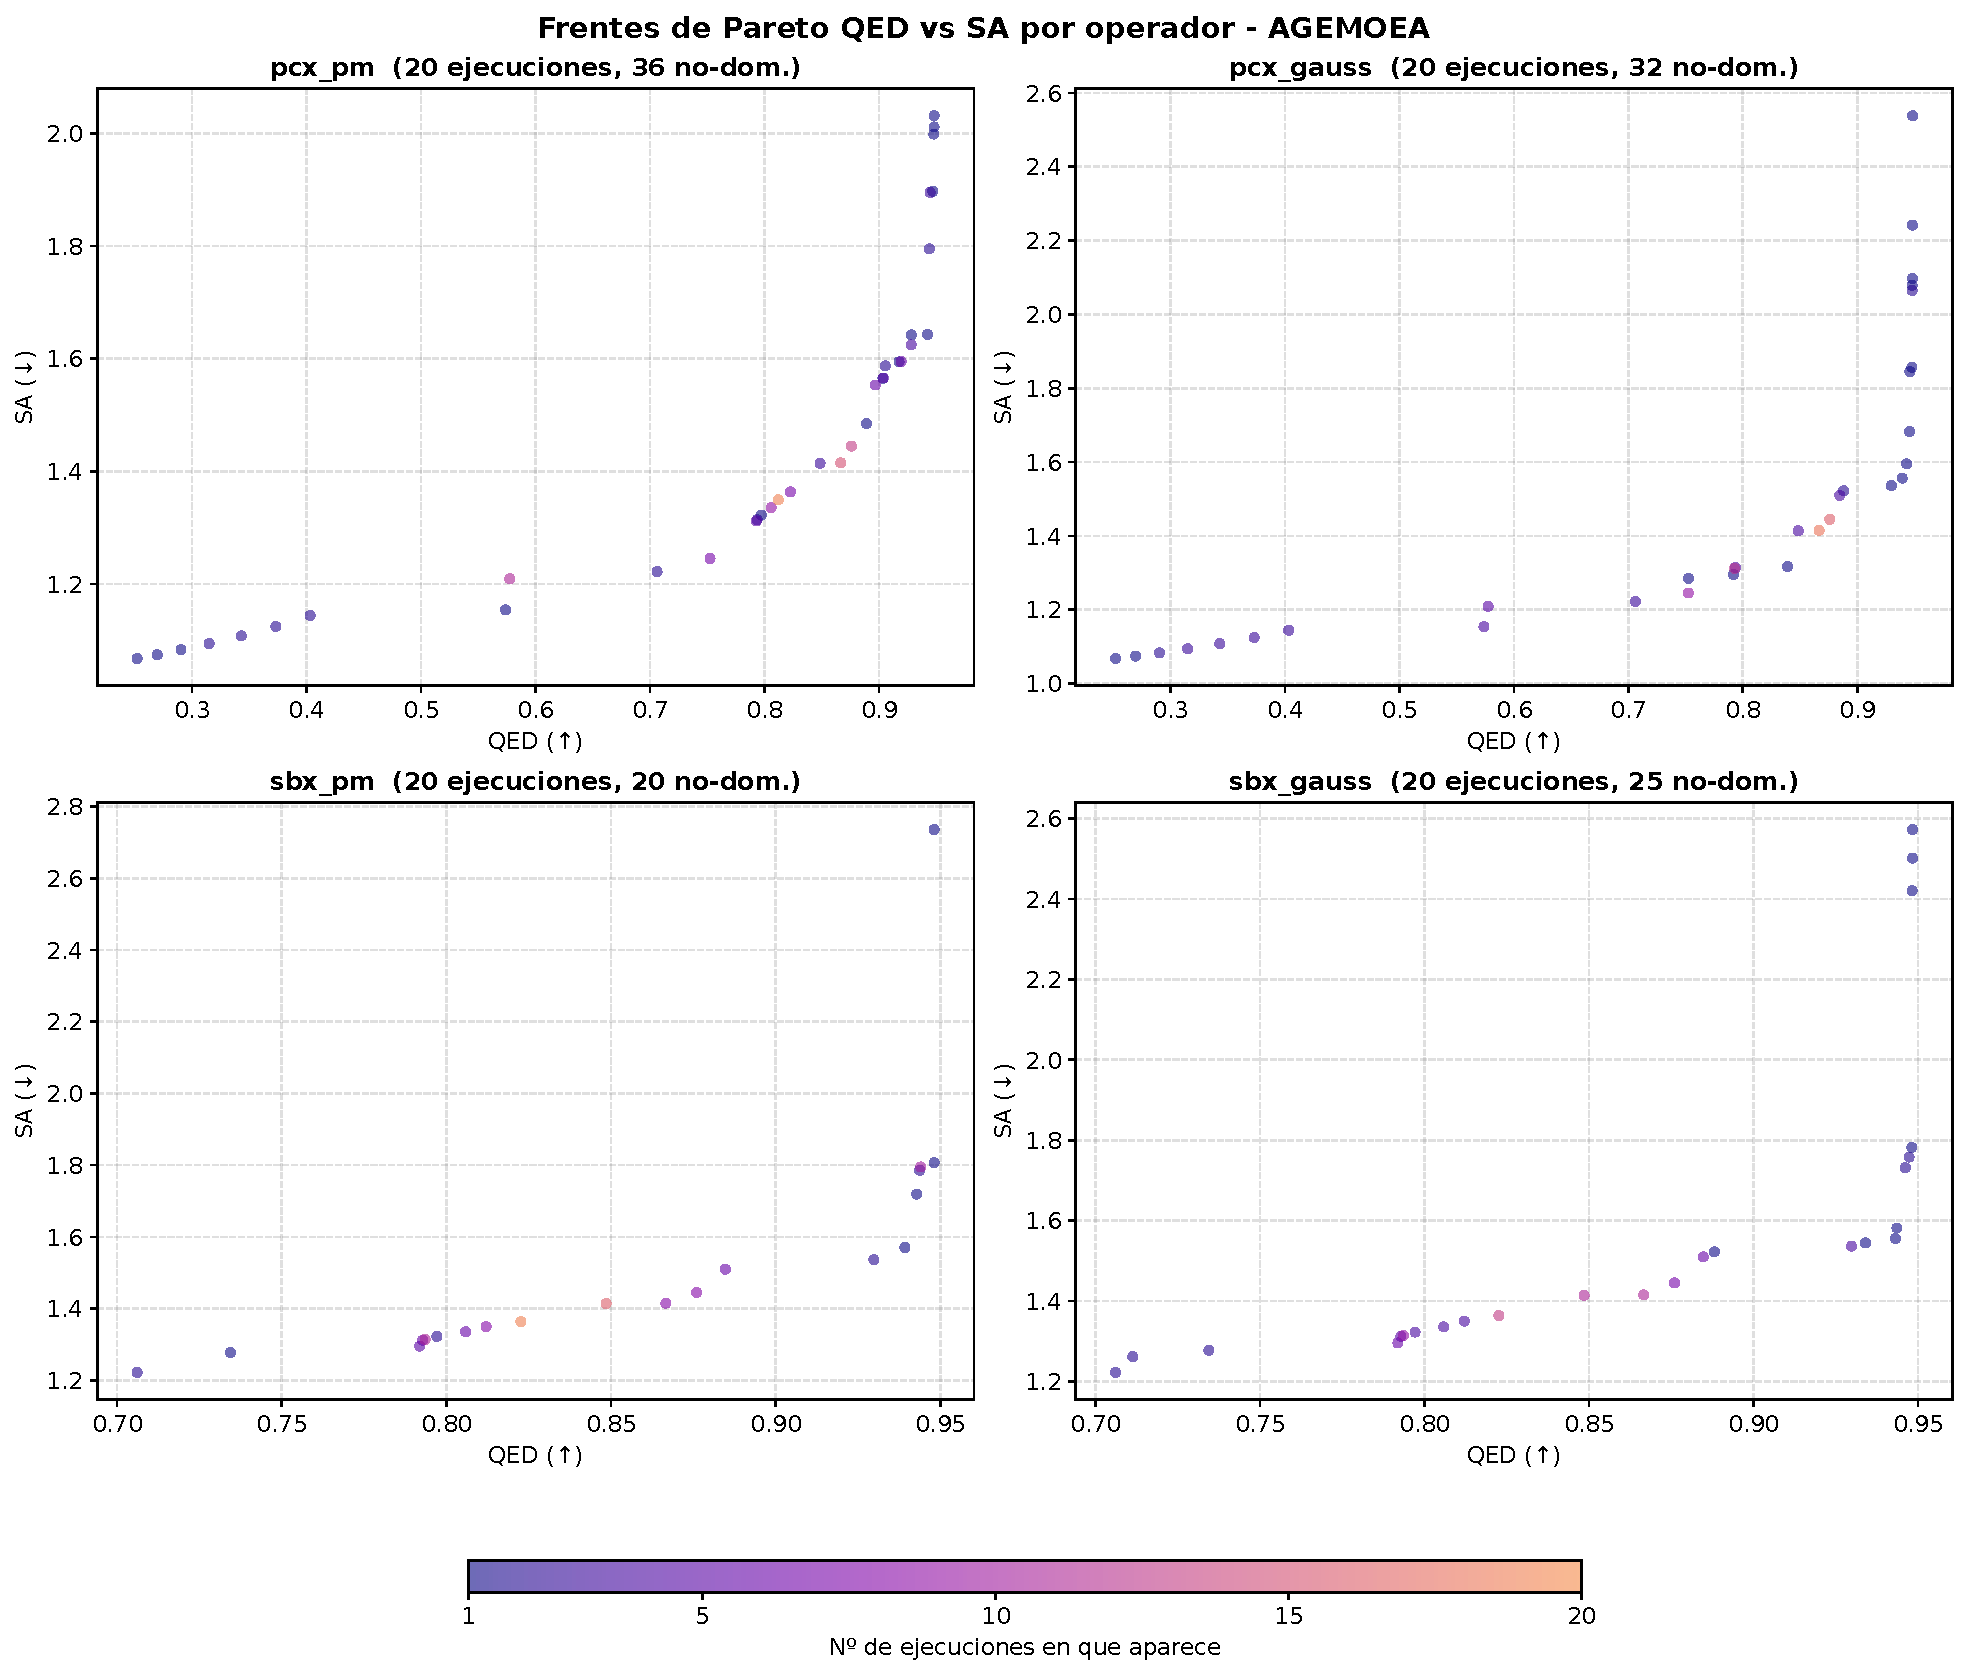
\includegraphics[width=0.95\textwidth]{Figures/metaheuristicas/operadores/AGEMOEA/pareto_qed_sa_grid_nruns_popAGEMOEA.pdf}
    \caption{Frentes no dominados acumulados sobre las veinte semillas en el espacio QED--SA para cada combinación de operadores en \acrshort{agemoea}, coloreados por el número de semillas en que apareció cada molécula.}
    \label{fig:pareto_agemoea_grid_nruns}
\end{figure}

\begin{figure}[H]
    \centering
    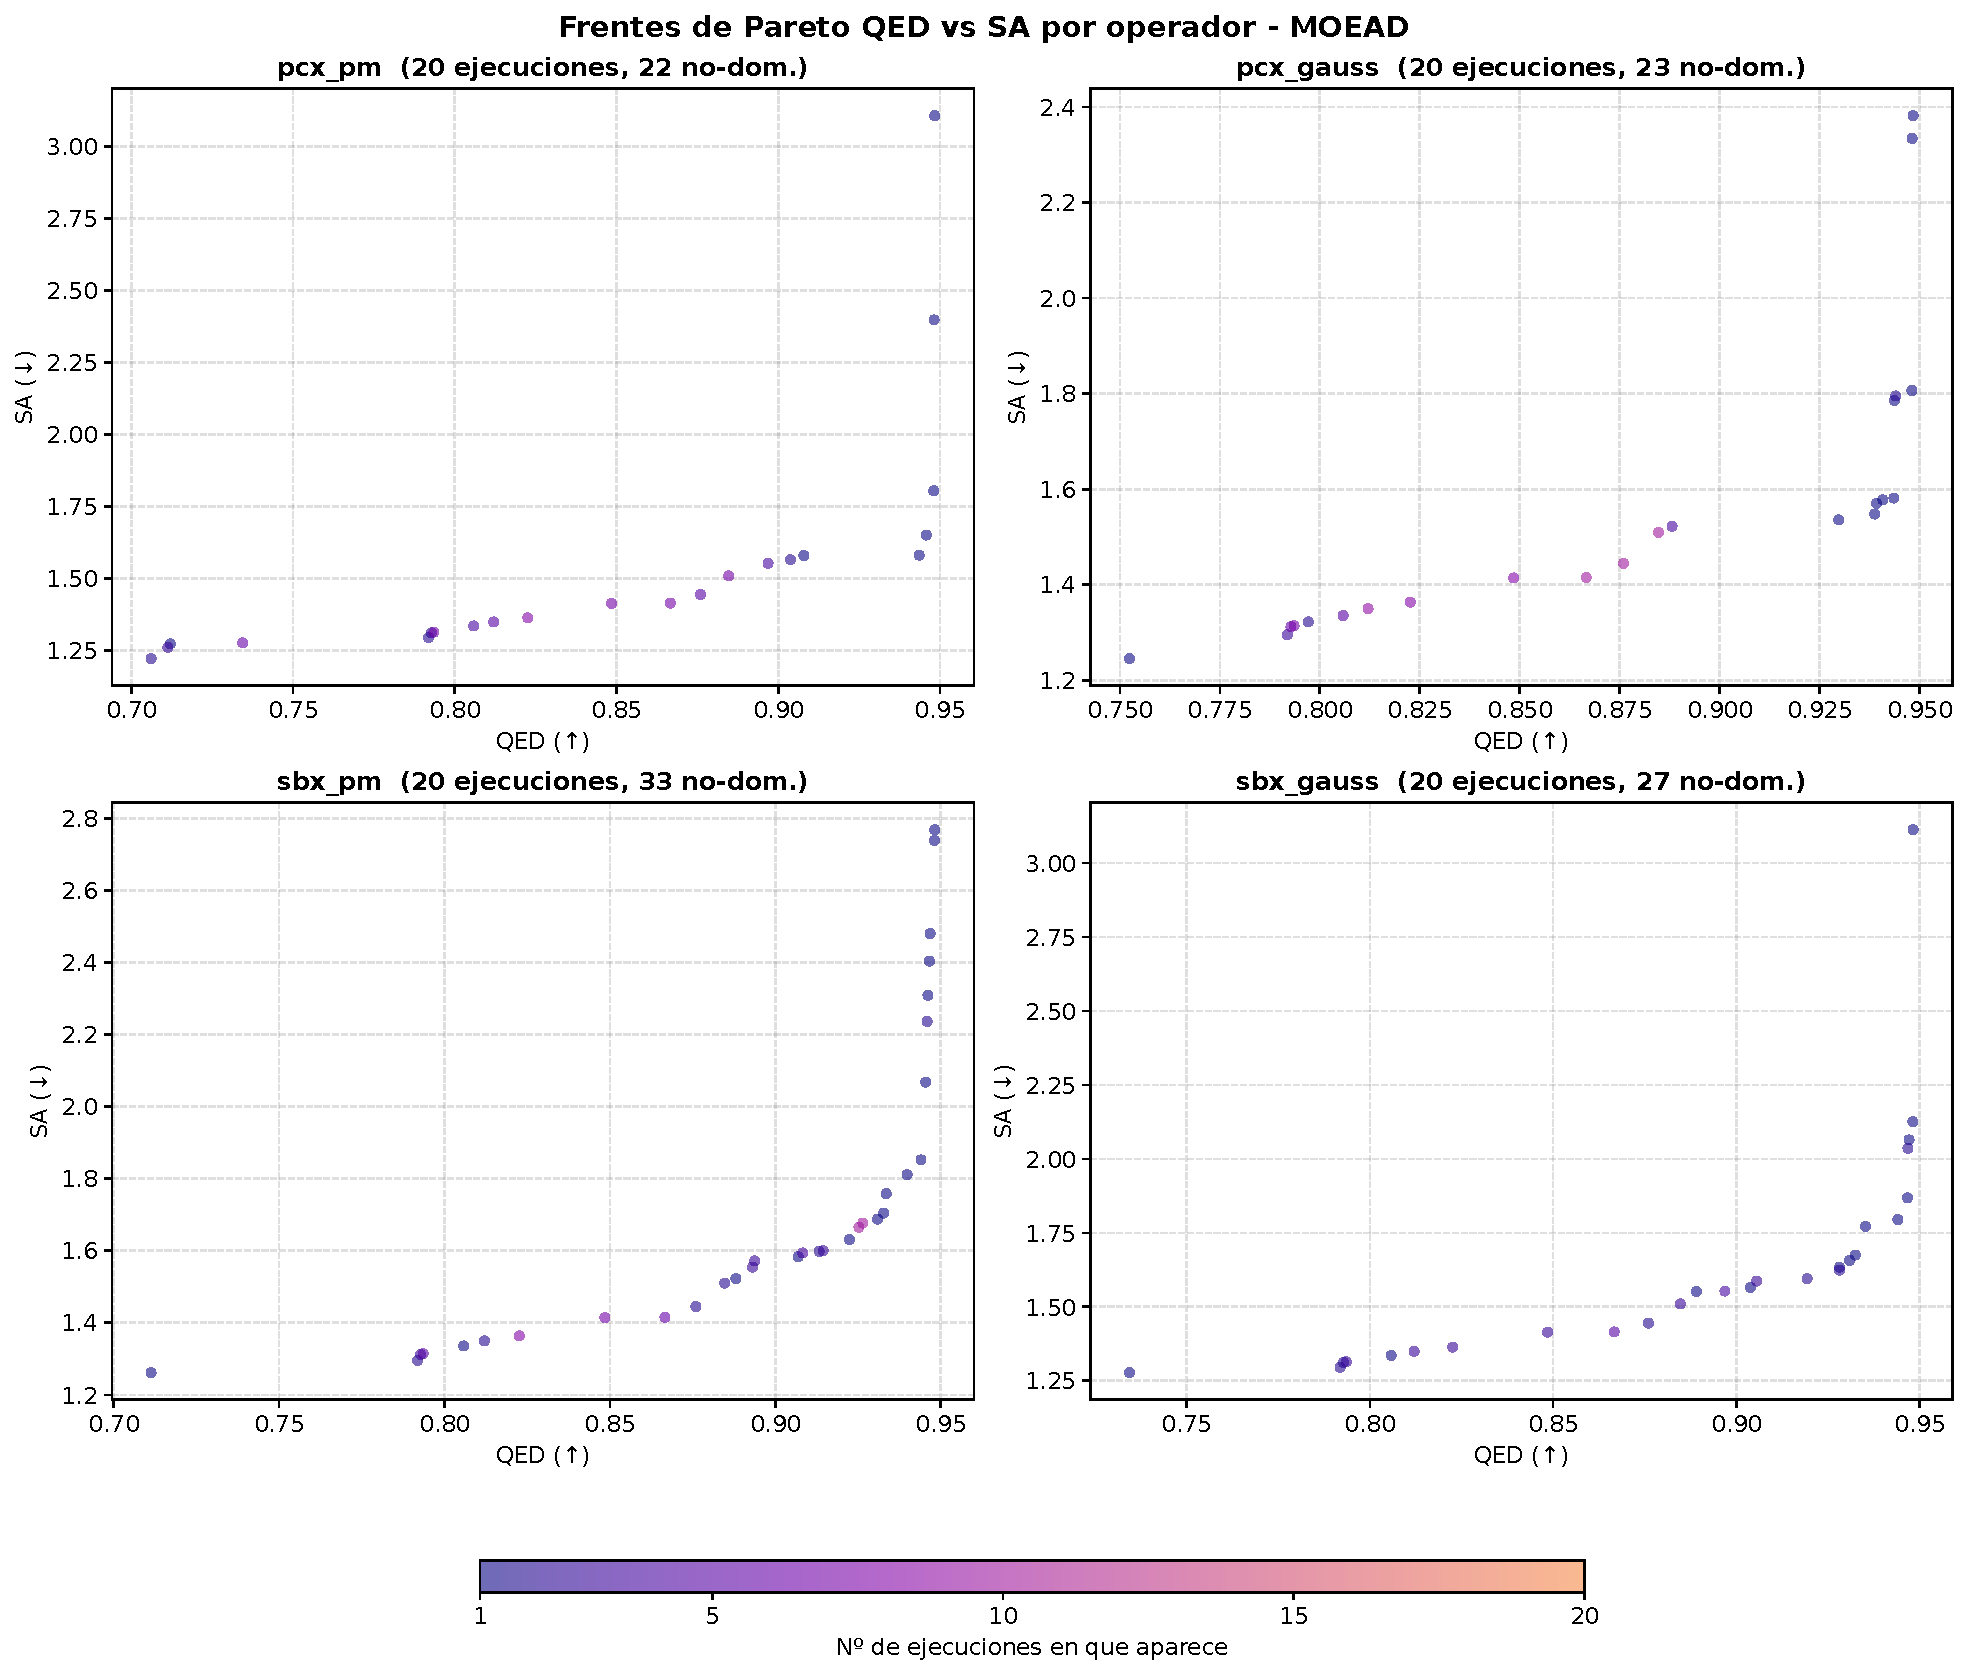
\includegraphics[width=0.95\textwidth]{Figures/metaheuristicas/operadores/MOEAD/pareto_qed_sa_grid_nruns_popMOEAD.pdf}
    \caption{Frentes no dominados acumulados sobre las veinte semillas en el espacio QED--SA para cada combinación de operadores en \acrshort{moead}, coloreados por el número de semillas en que apareció cada molécula.}
    \label{fig:pareto_moead_grid_nruns}
\end{figure}

\begin{figure}[H]
    \centering
    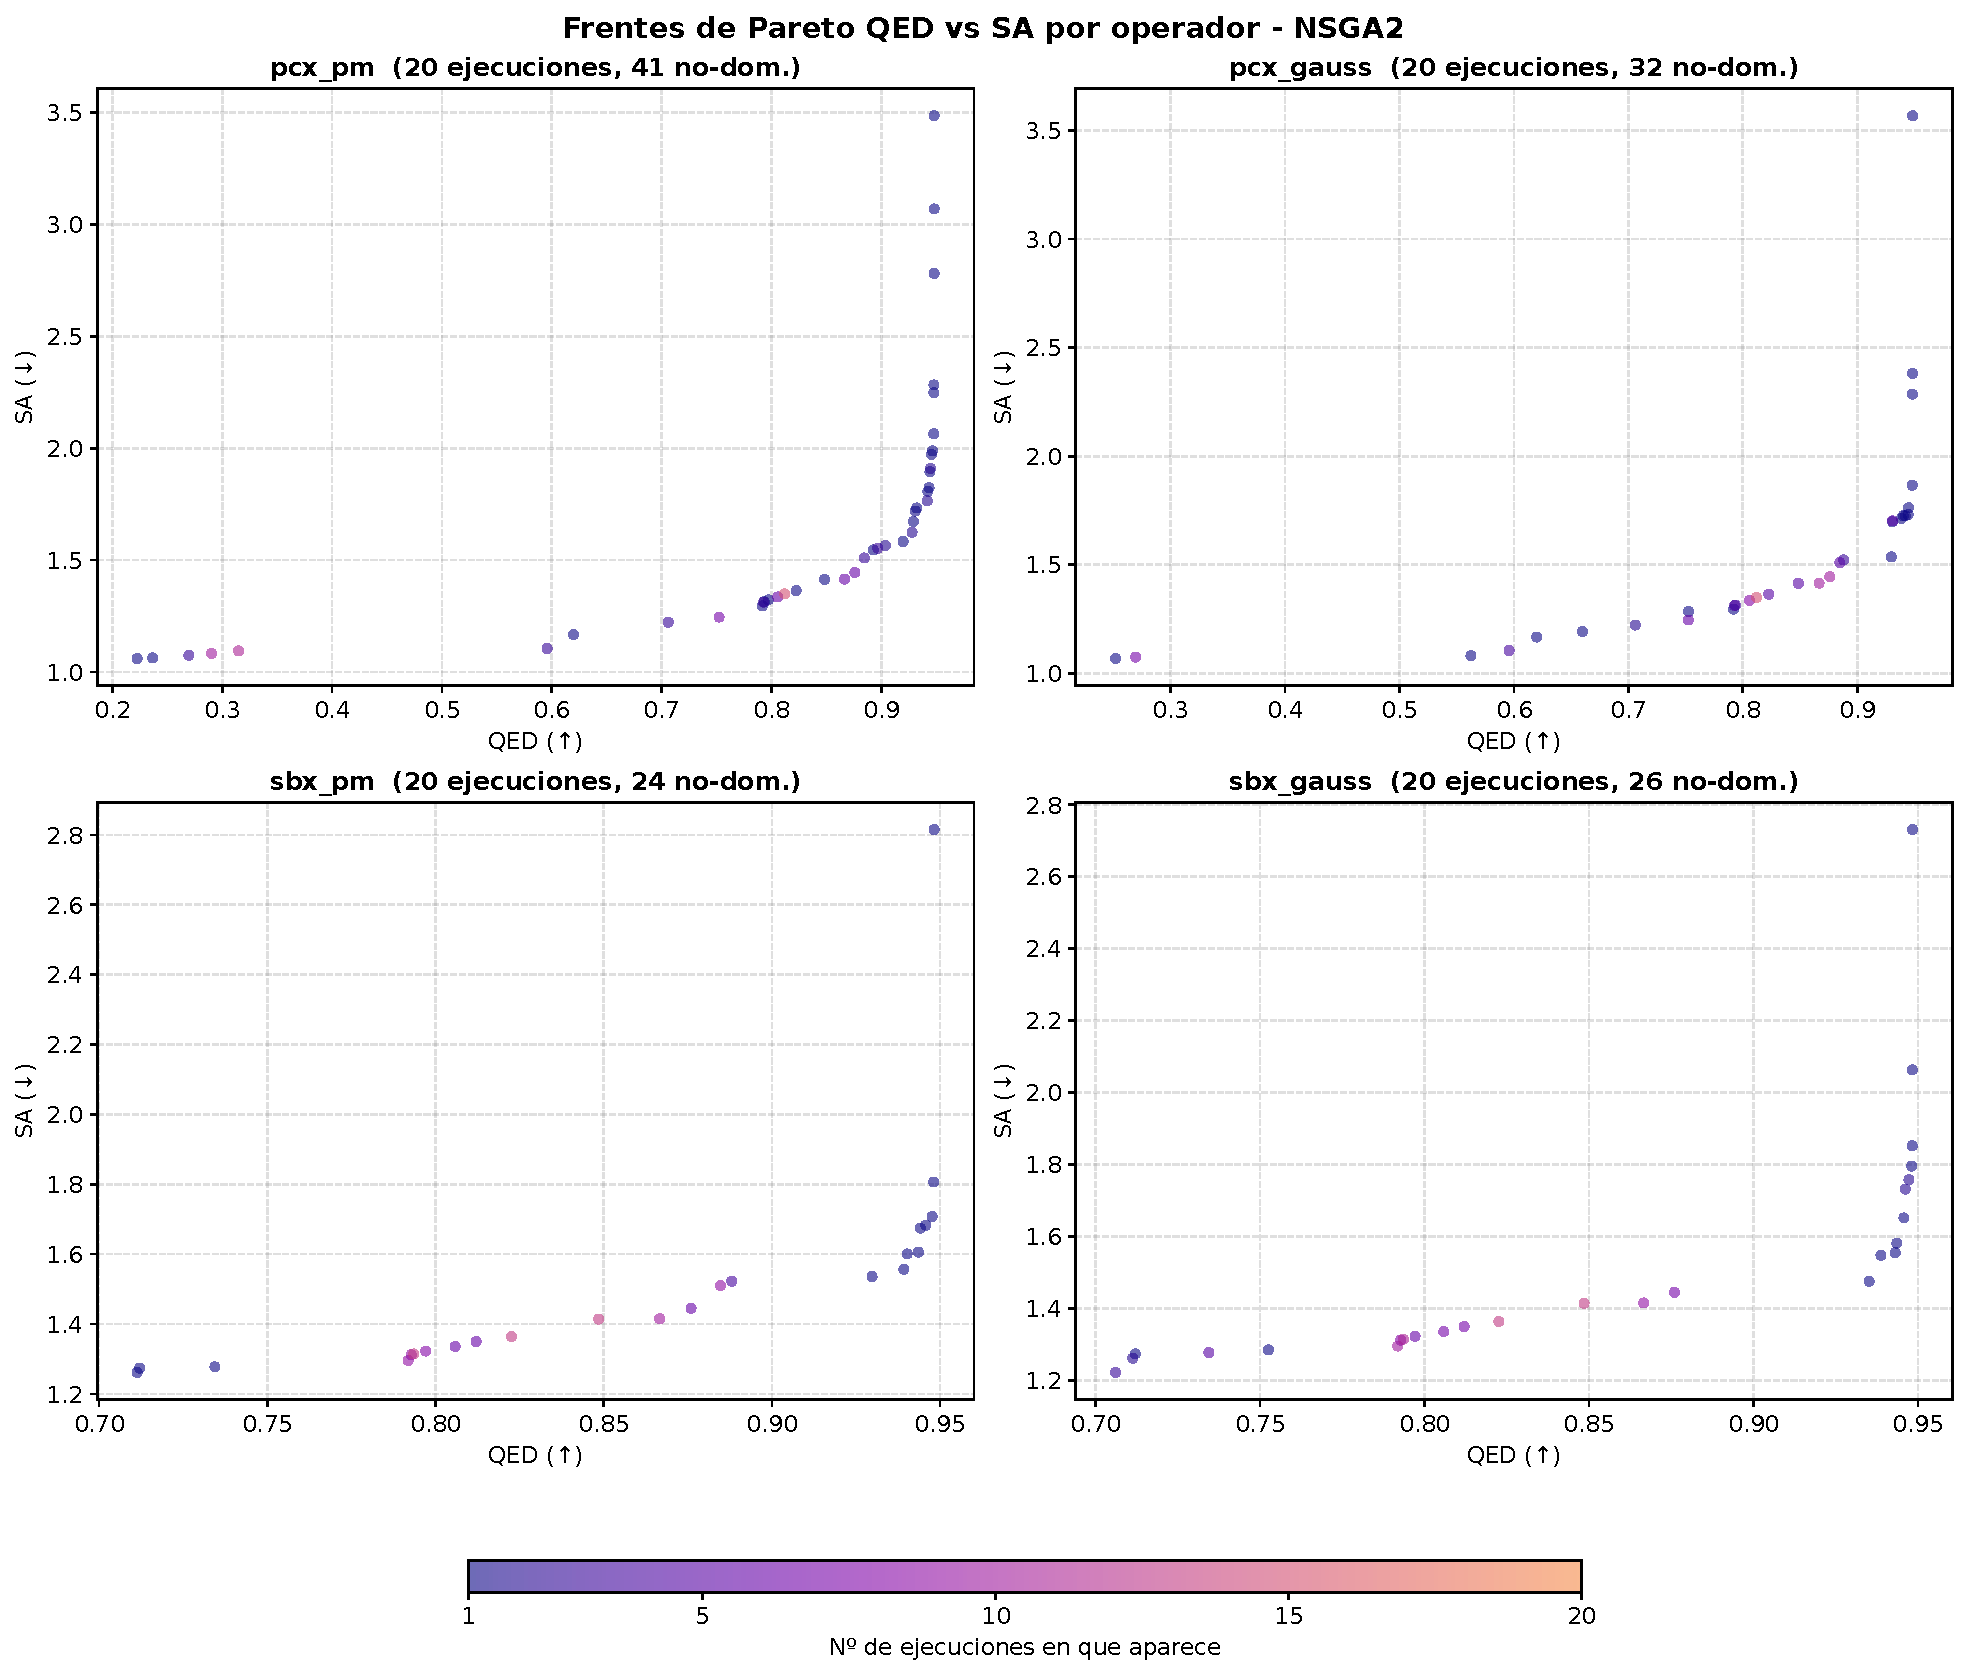
\includegraphics[width=0.95\textwidth]{Figures/metaheuristicas/operadores/NSGA2/pareto_qed_sa_grid_nruns_popNSGA2.pdf}
    \caption{Frentes no dominados acumulados sobre las veinte semillas en el espacio QED--SA para cada combinación de operadores en \acrshort{nsga2}, coloreados por el número de semillas en que apareció cada molécula.}
    \label{fig:pareto_nsga2_grid_nruns}
\end{figure}

\begin{figure}[H]
    \centering
    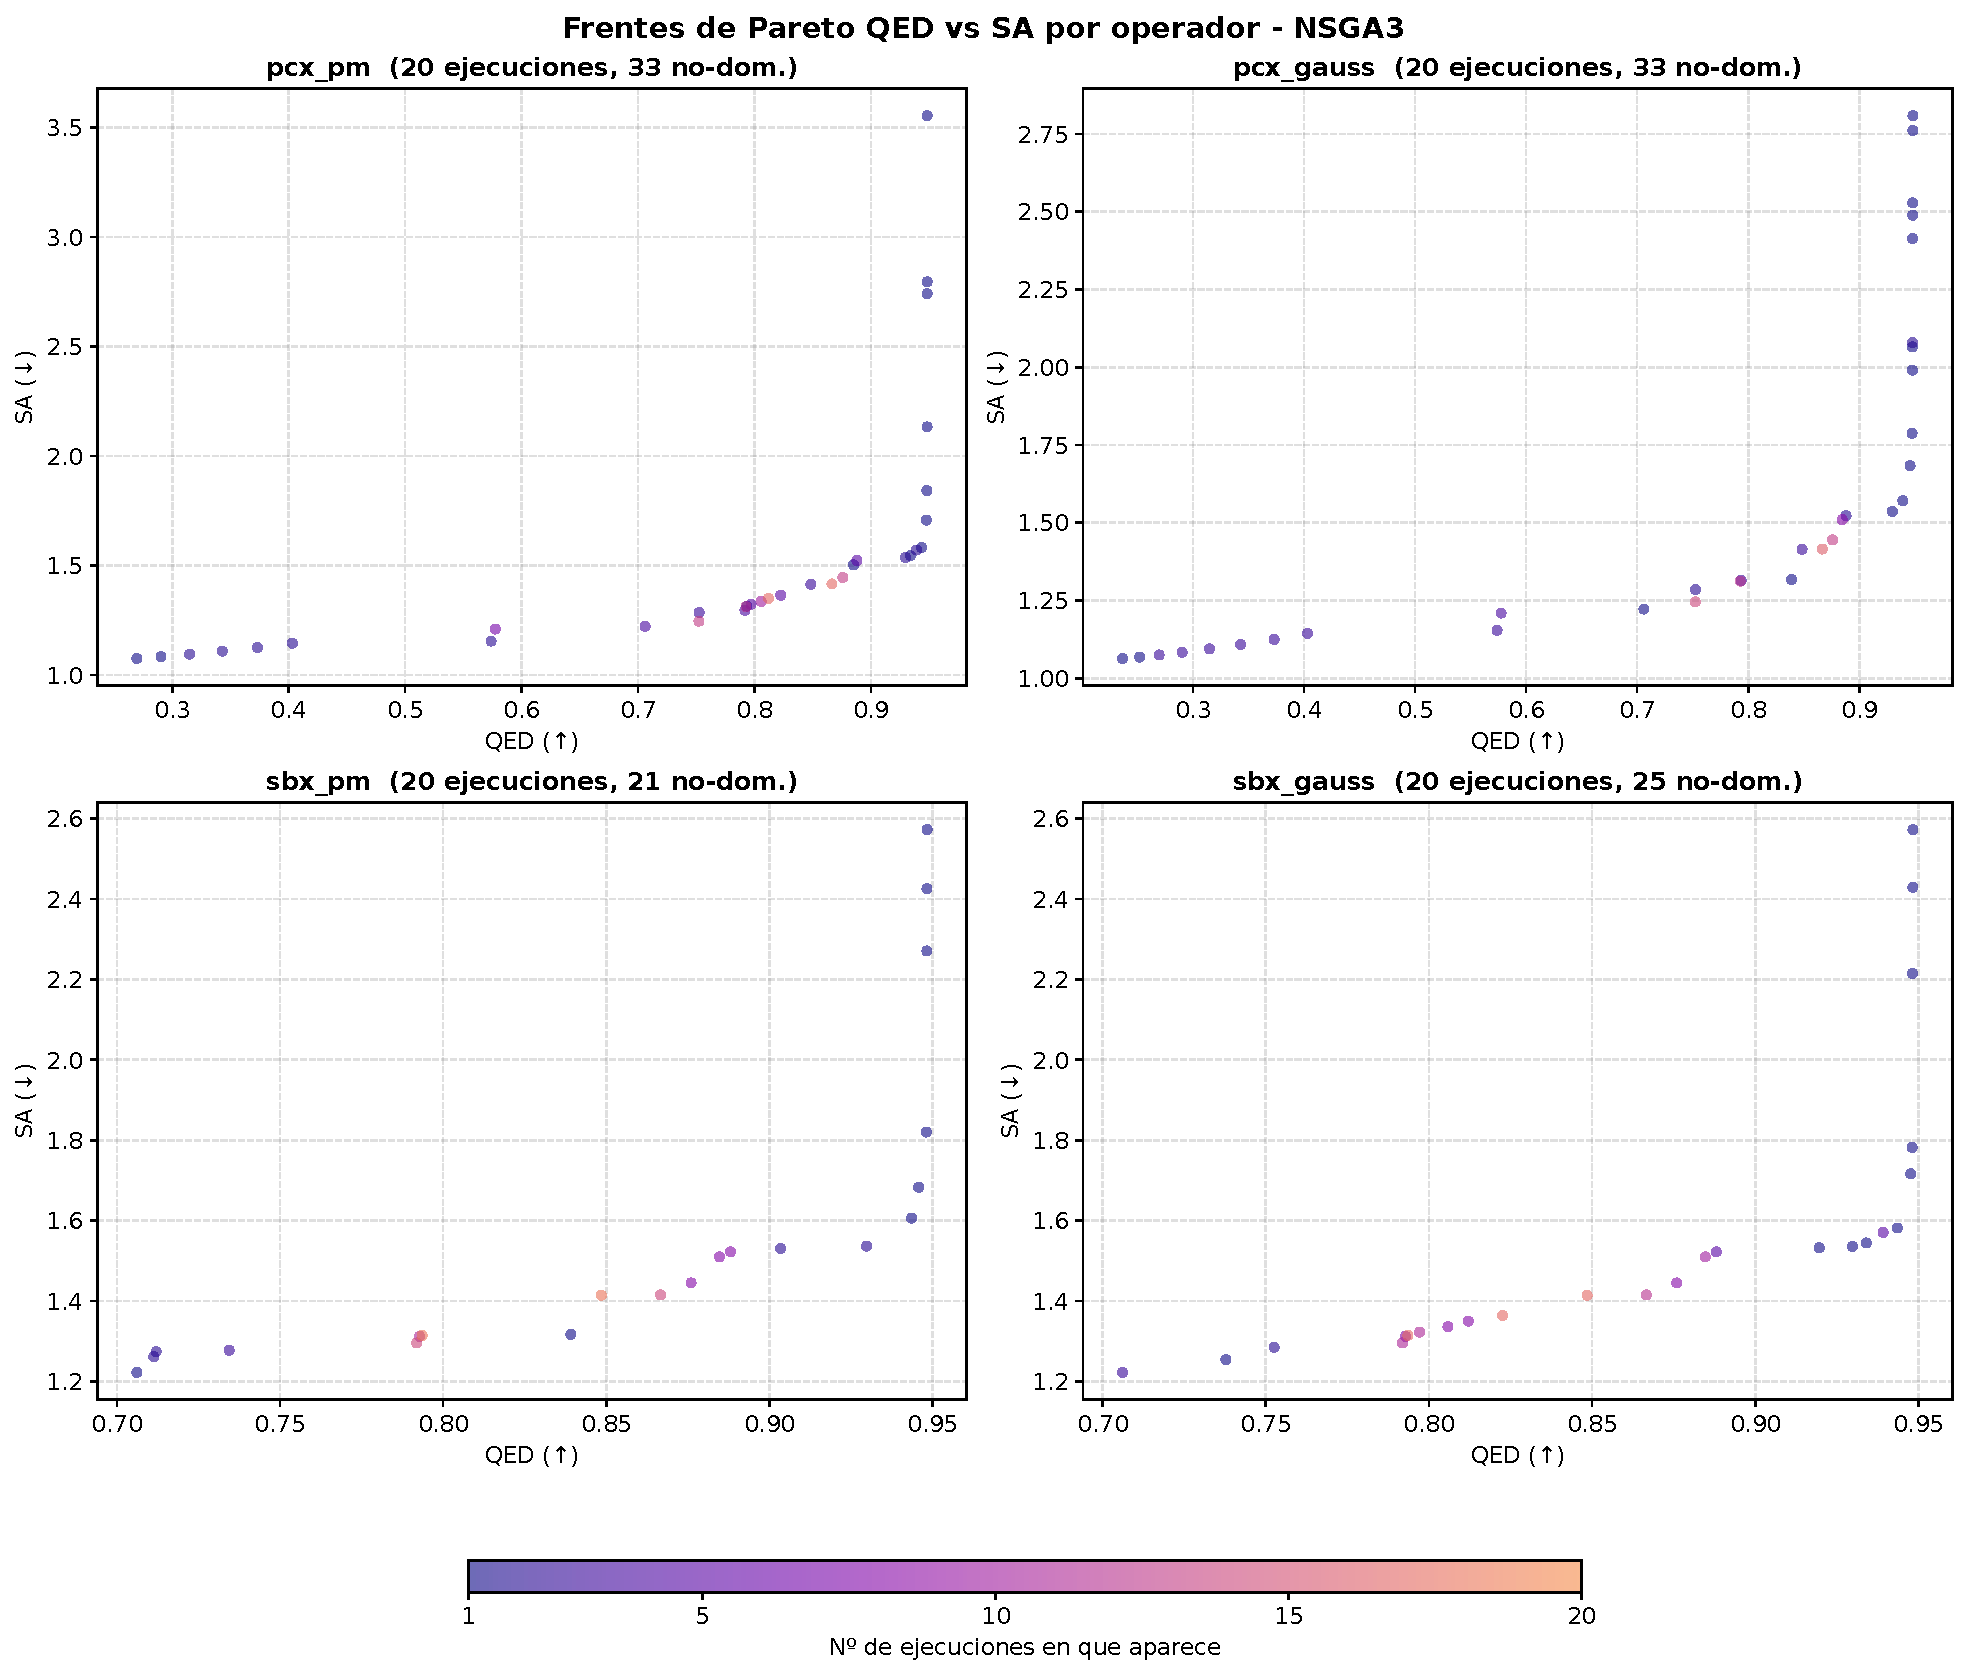
\includegraphics[width=0.95\textwidth]{Figures/metaheuristicas/operadores/NSGA3/pareto_qed_sa_grid_nruns_popNSGA3.pdf}
    \caption{Frentes no dominados acumulados sobre las veinte semillas en el espacio QED--SA para cada combinación de operadores en \acrshort{nsga3}, coloreados por el número de semillas en que apareció cada molécula.}
    \label{fig:pareto_nsga3_grid_nruns}
\end{figure}

\clearpage
\section{Estructuras Químicas Obtenidas por Combinación de Operadores}
\label{sec:apendice_moleculas_operadores}

\begin{figure}[H]
    \centering
    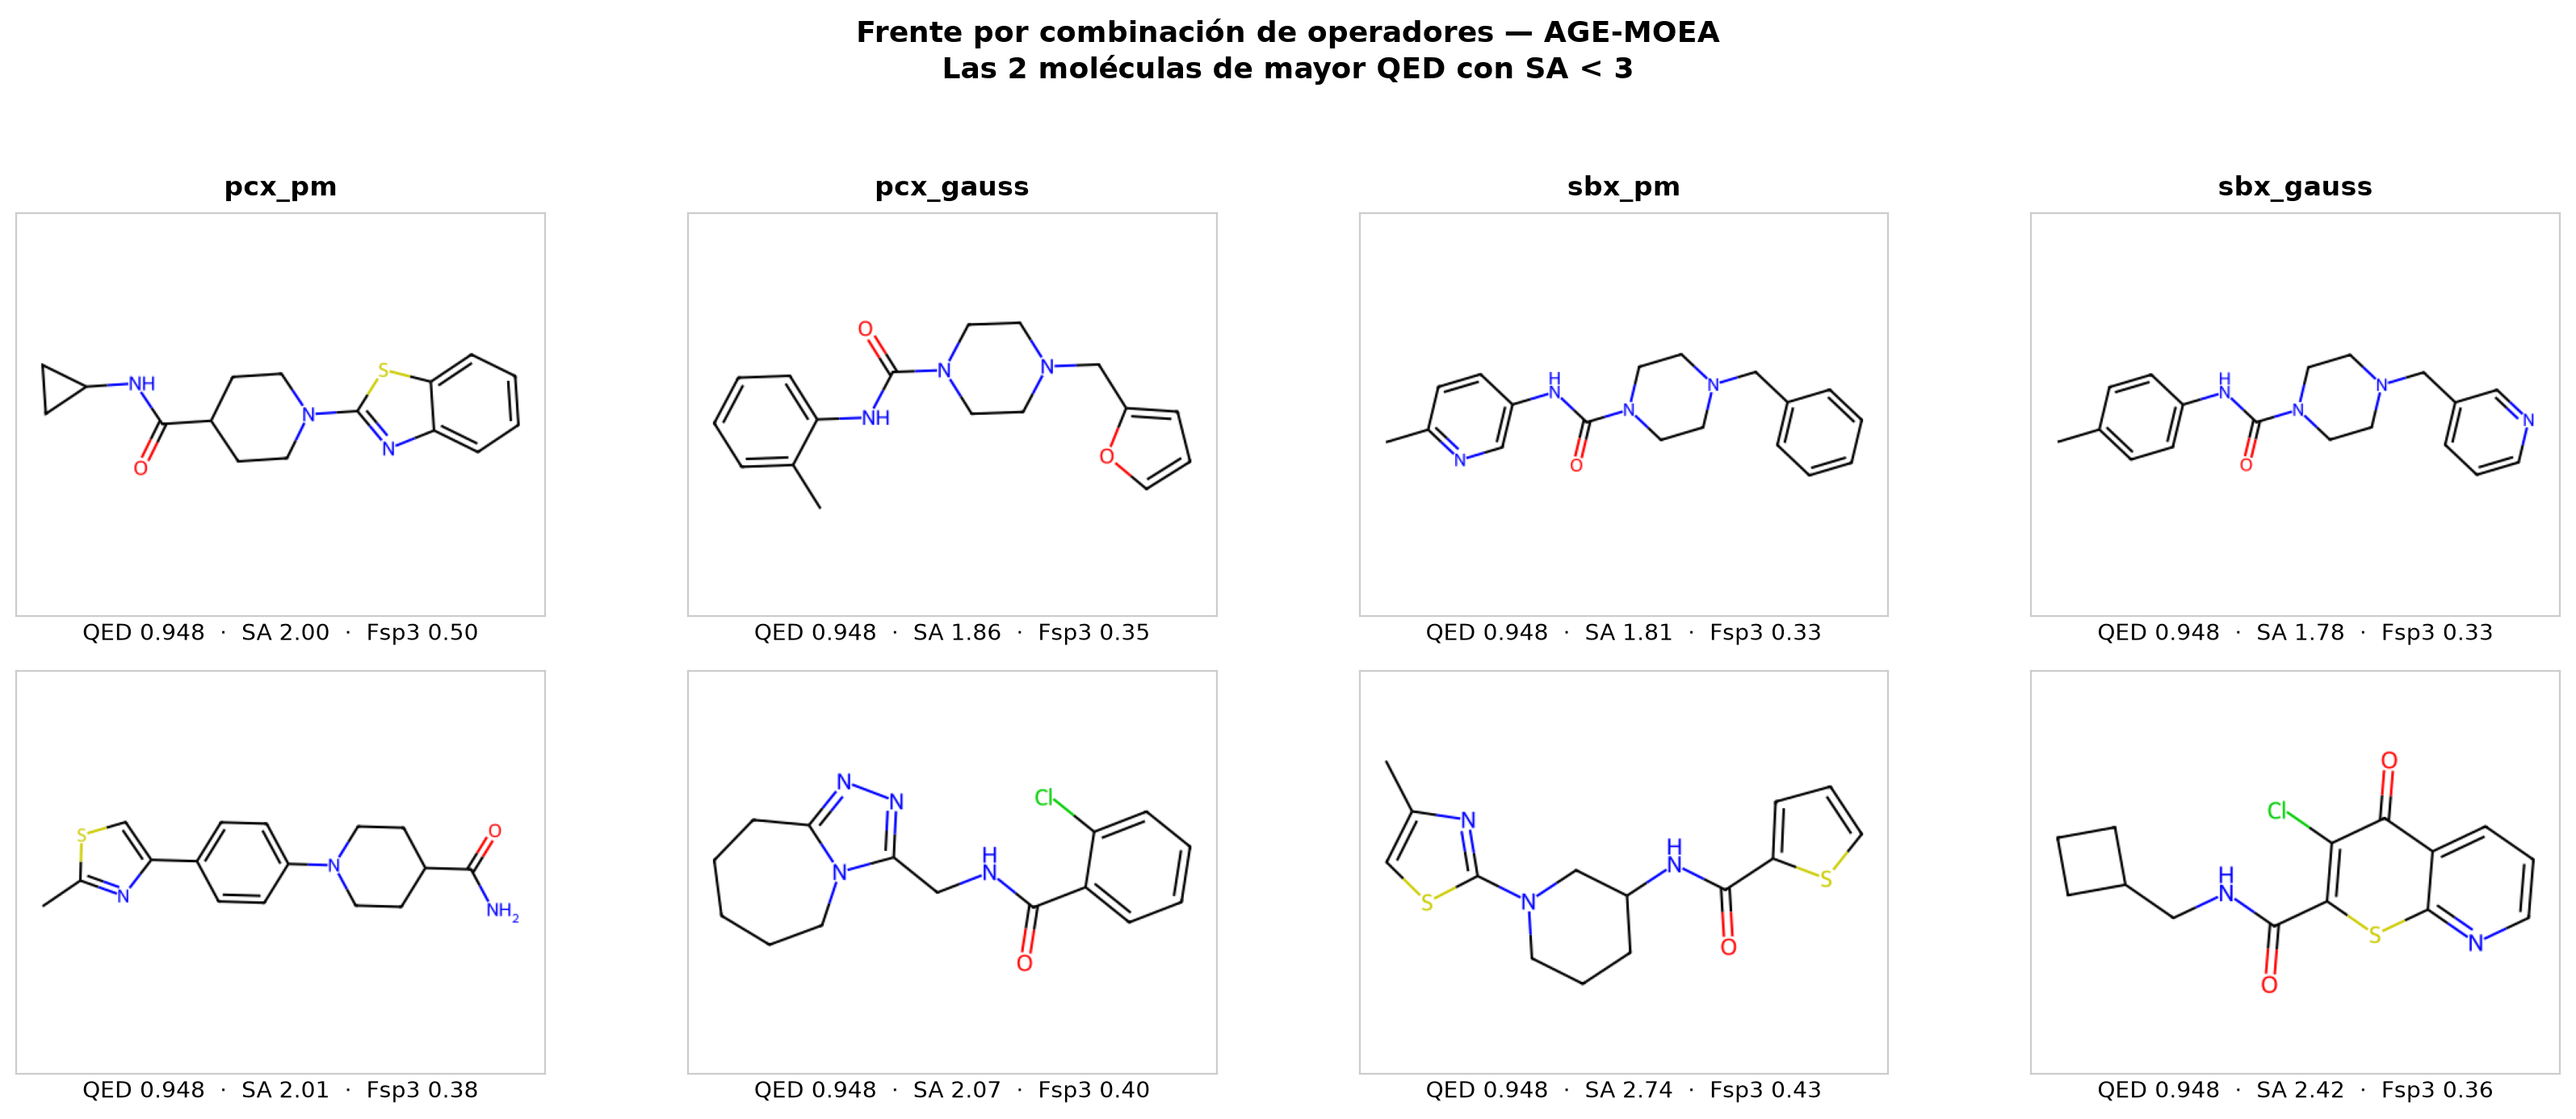
\includegraphics[width=0.95\textwidth]{Figures/metaheuristicas/operadores/AGEMOEA/moleculas_operadores_AGEMOEA.png}
    \caption{Moléculas de mayor QED con $\text{SA} < 3$ seleccionadas del frente no dominado acumulado para cada combinación de operadores en \acrshort{agemoea}.}
    \label{fig:moleculas_operadores_agemoea}
\end{figure}

\begin{figure}[H]
    \centering
    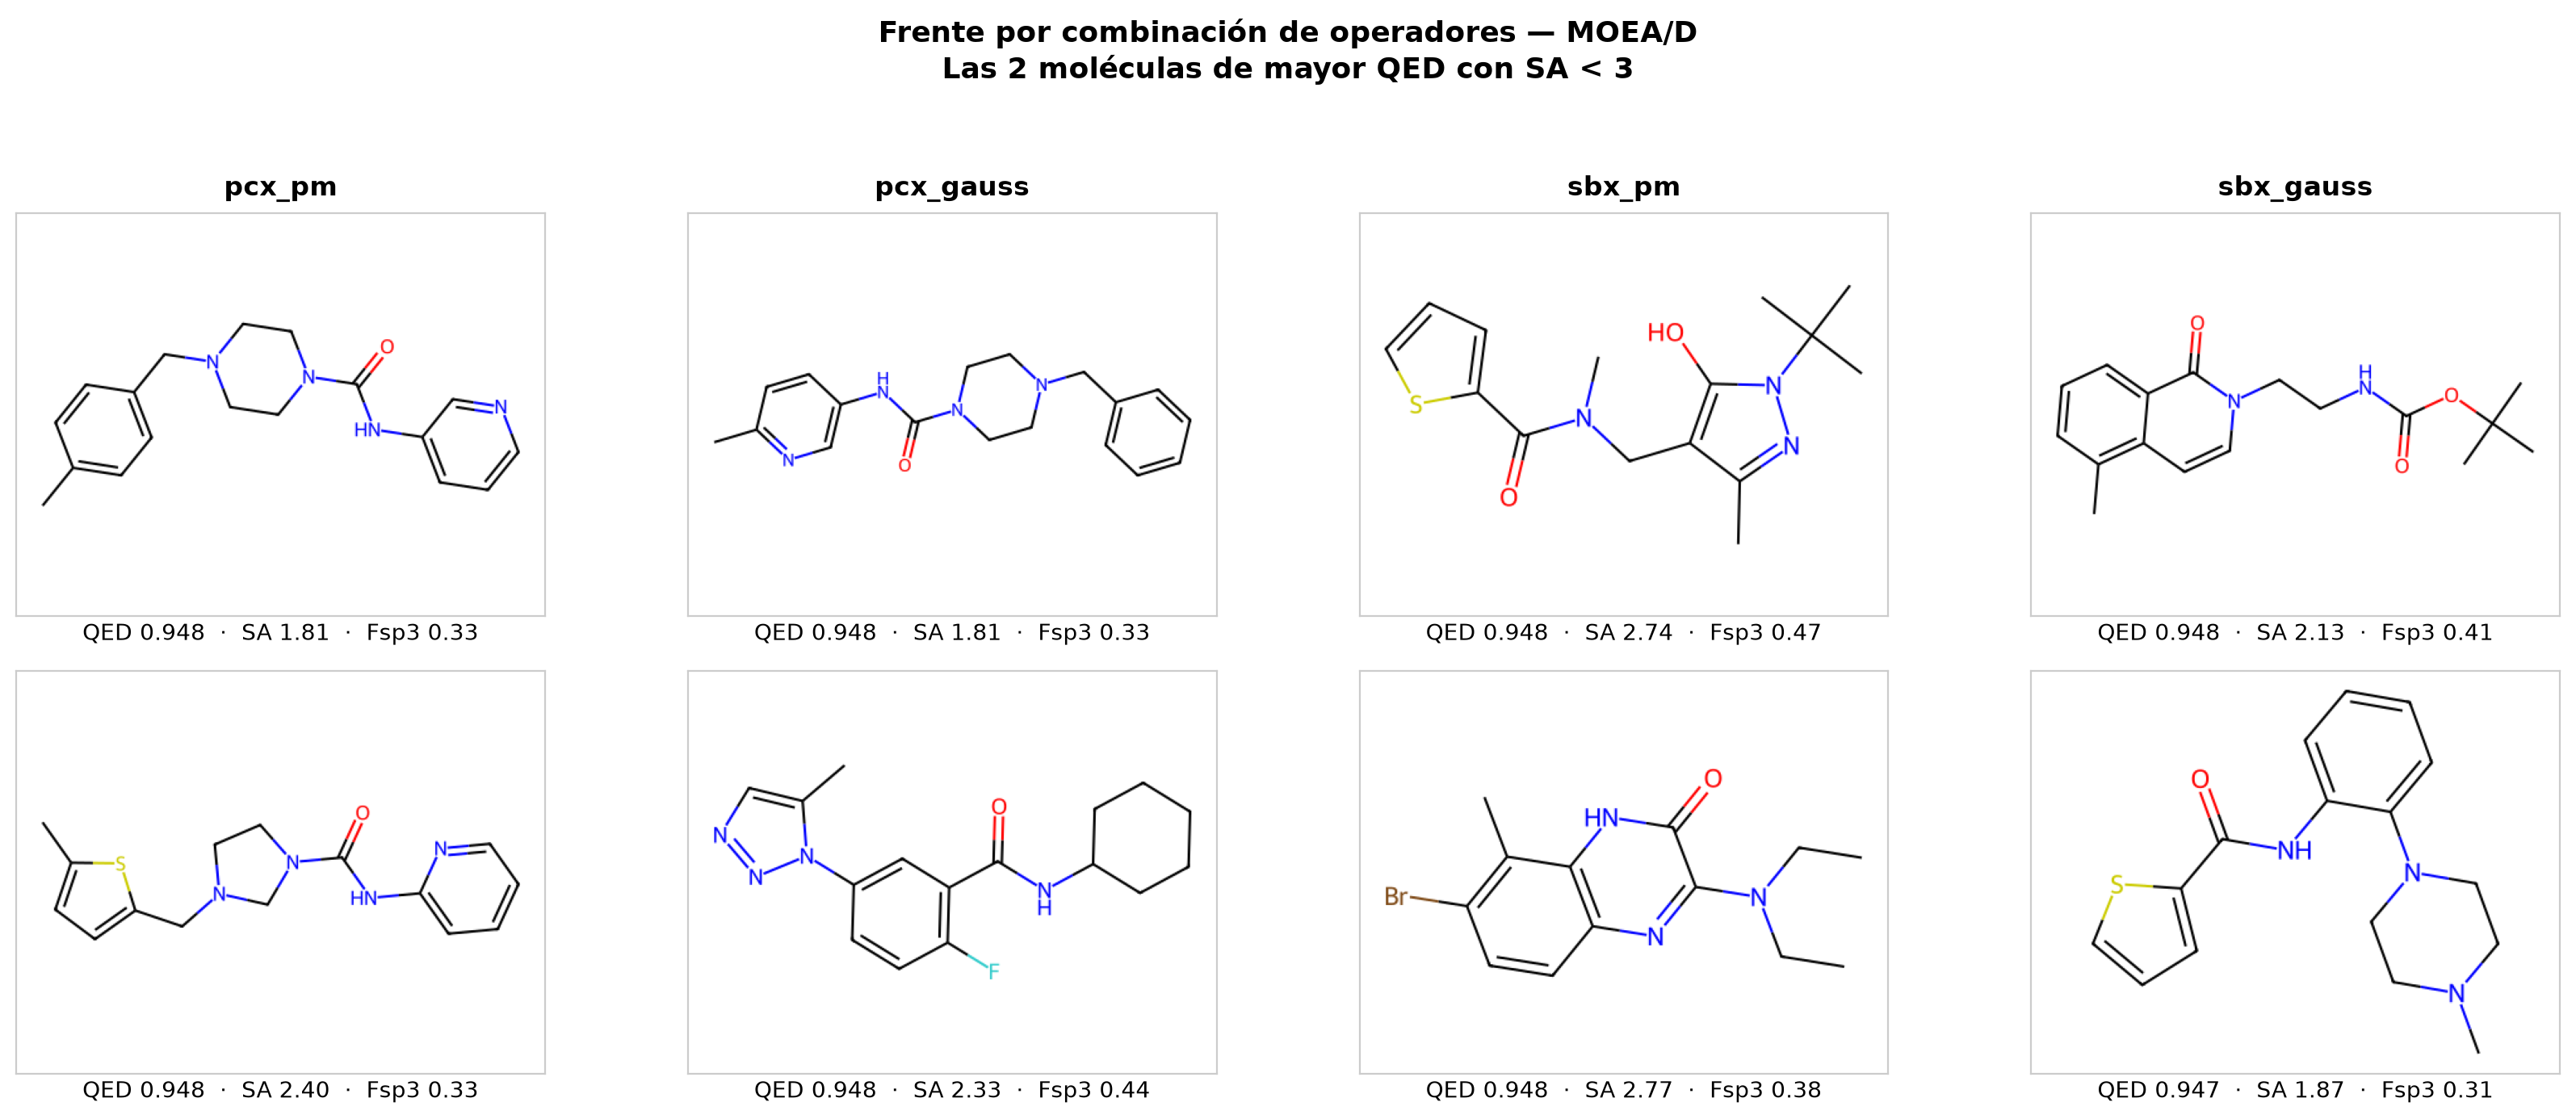
\includegraphics[width=0.95\textwidth]{Figures/metaheuristicas/operadores/MOEAD/moleculas_operadores_MOEAD.png}
    \caption{Moléculas de mayor QED con $\text{SA} < 3$ seleccionadas del frente no dominado acumulado para cada combinación de operadores en \acrshort{moead}.}
    \label{fig:moleculas_operadores_moead}
\end{figure}

\begin{figure}[H]
    \centering
    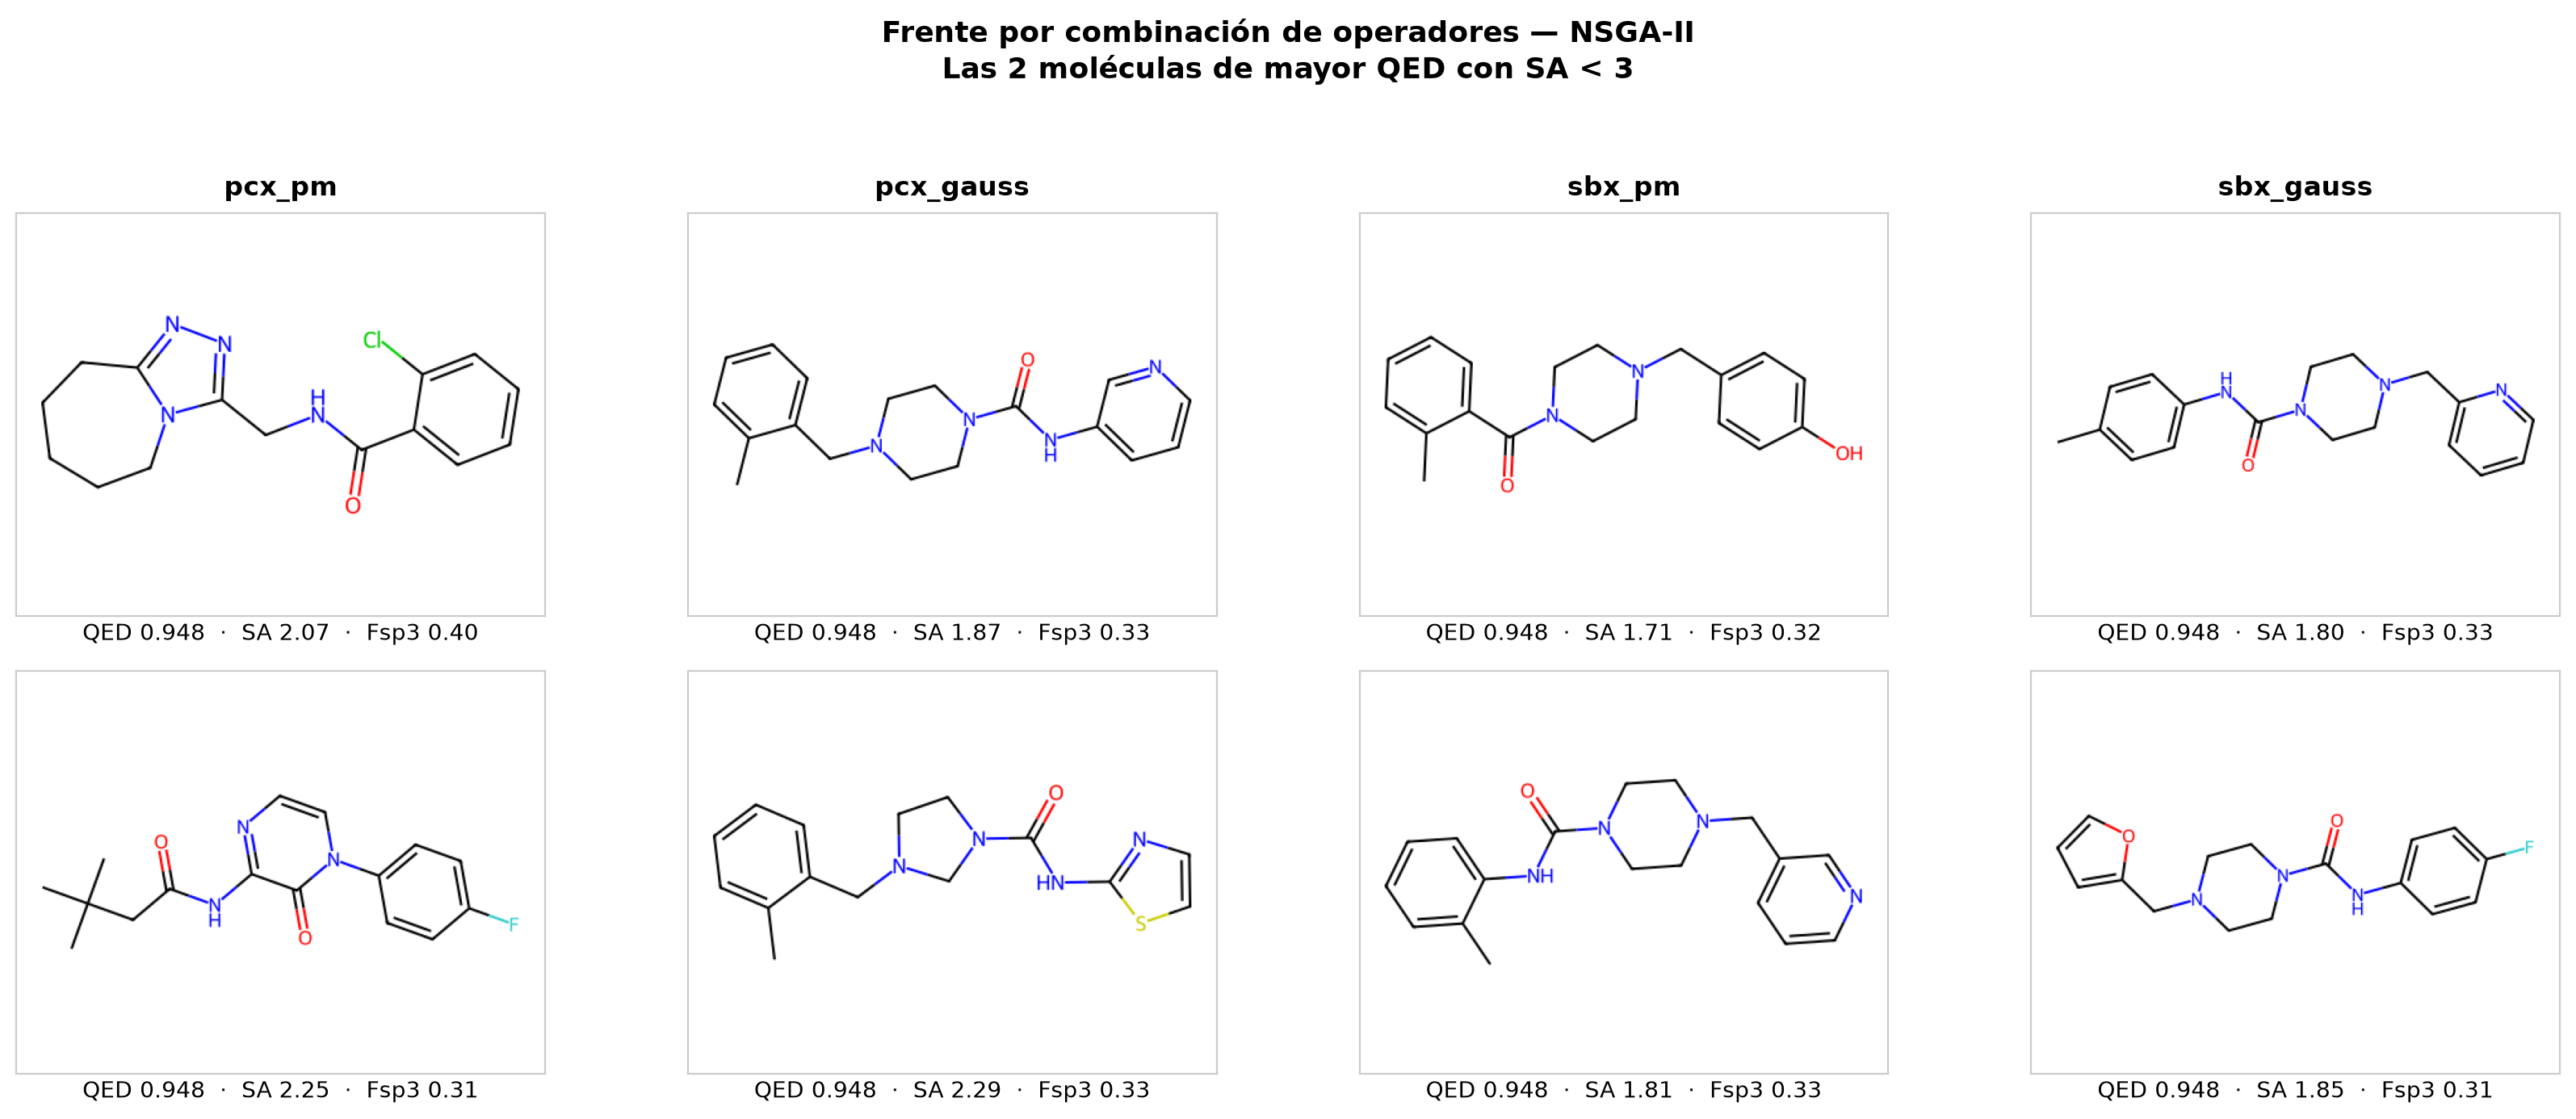
\includegraphics[width=0.95\textwidth]{Figures/metaheuristicas/operadores/NSGA2/moleculas_operadores_NSGA2.png}
    \caption{Moléculas de mayor QED con $\text{SA} < 3$ seleccionadas del frente no dominado acumulado para cada combinación de operadores en \acrshort{nsga2}.}
    \label{fig:moleculas_operadores_nsga2}
\end{figure}

\begin{figure}[H]
    \centering
    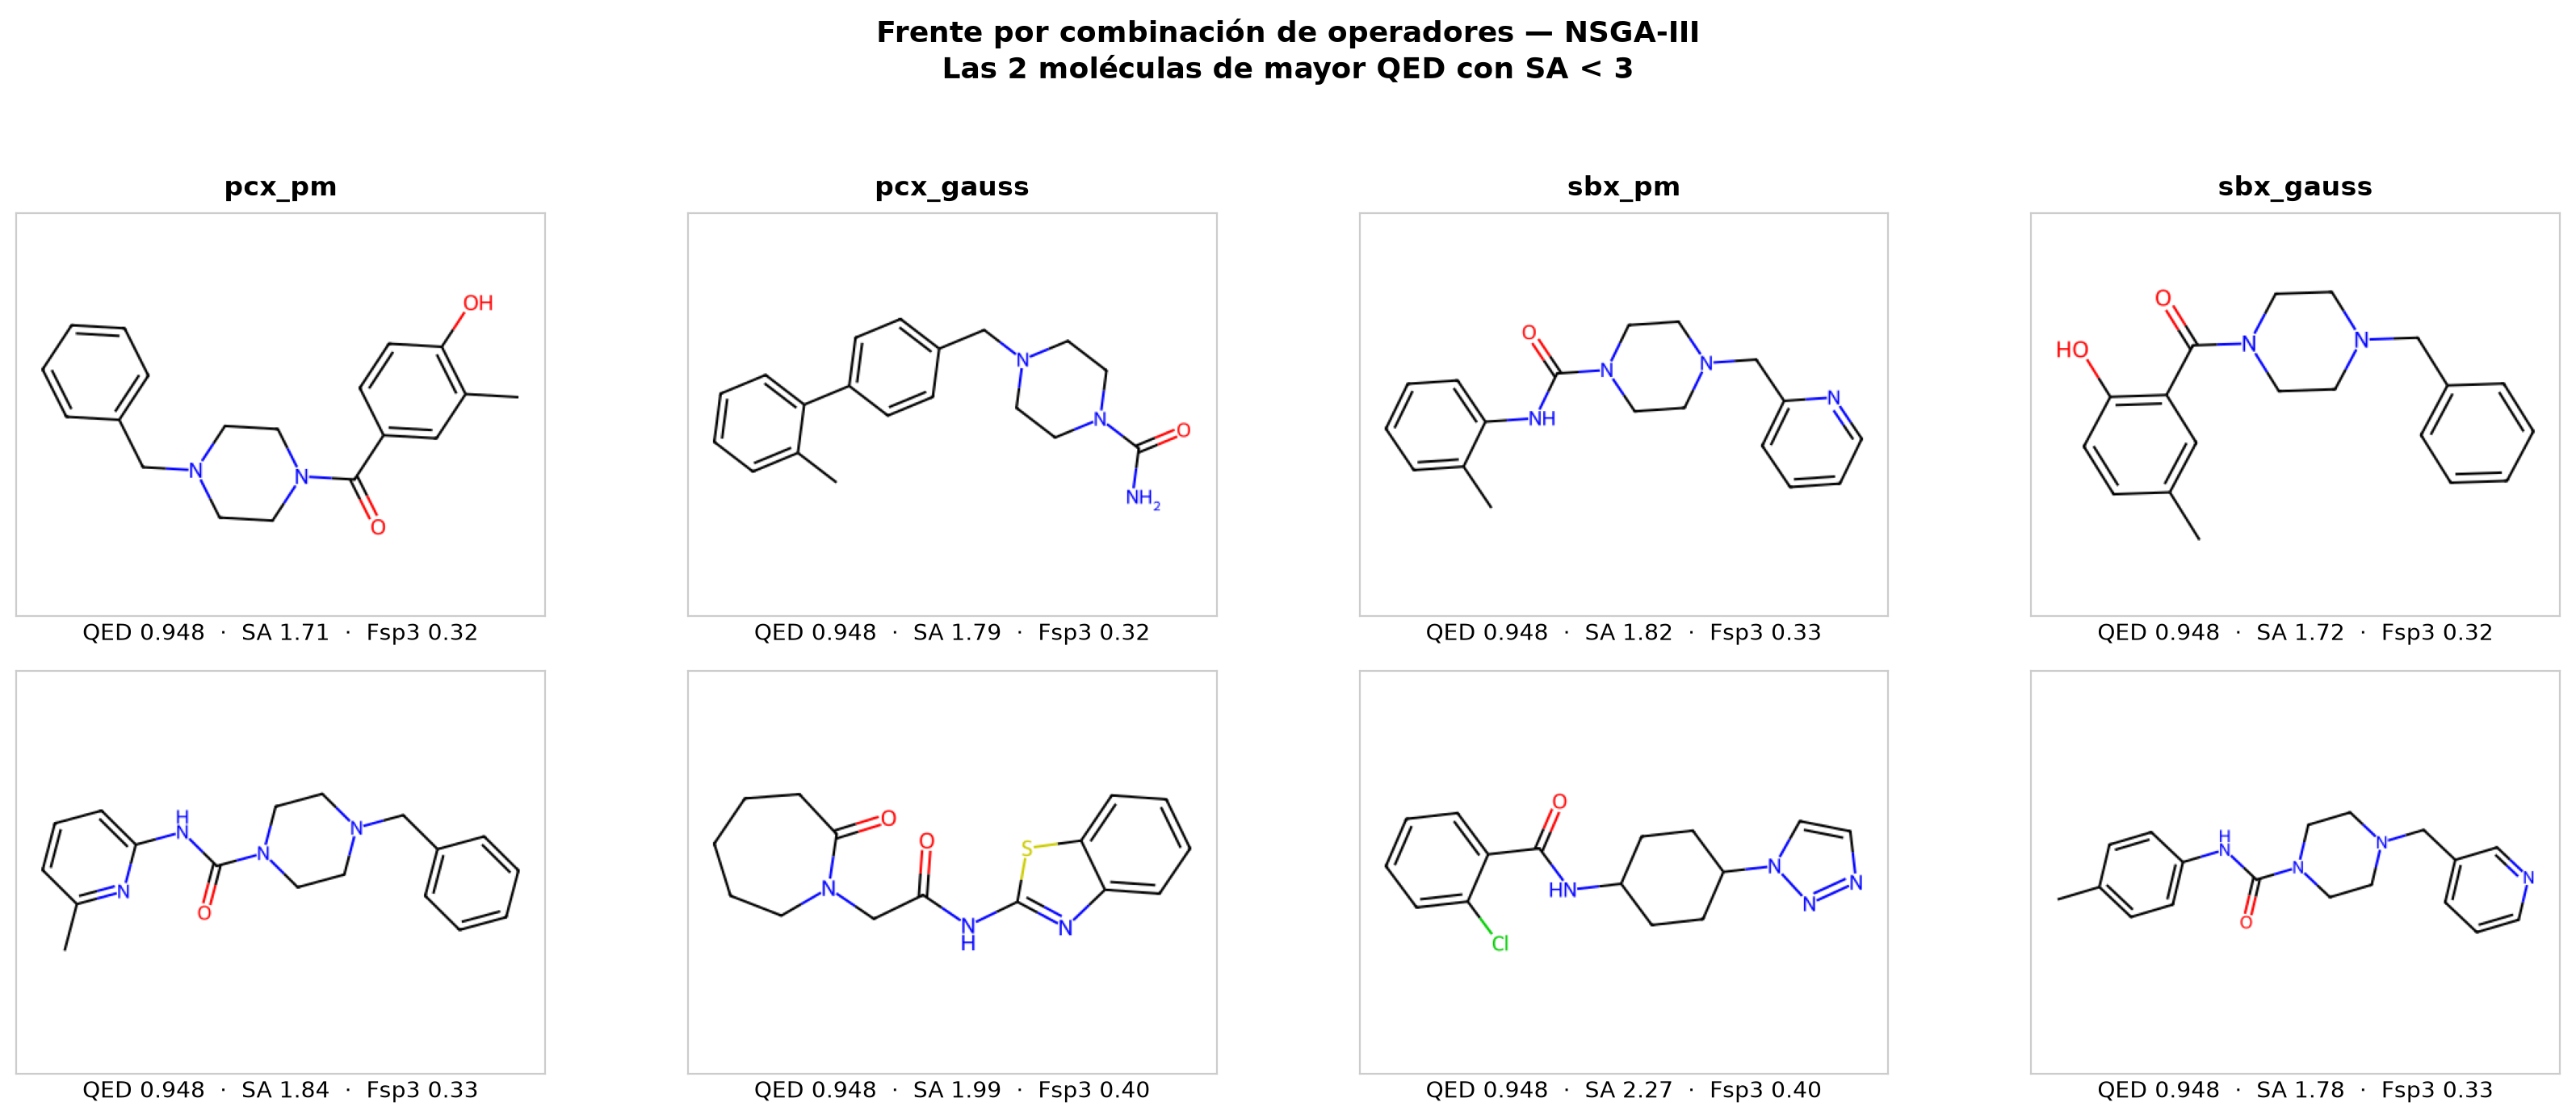
\includegraphics[width=0.95\textwidth]{Figures/metaheuristicas/operadores/NSGA3/moleculas_operadores_NSGA3.png}
    \caption{Moléculas de mayor QED con $\text{SA} < 3$ seleccionadas del frente no dominado acumulado para cada combinación de operadores en \acrshort{nsga3}.}
    \label{fig:moleculas_operadores_nsga3}
\end{figure}
